% \begin{document}
\chapter{Linear Programming}
\section{Introduction}
A linear programing problem is the problem of finding values for variables that optimize a given
linear objective function, subject to linear constraints.

Let us state an example of a linear program:
\begin{center}
\begin{tabular}{ll}
  Maximize   & $x+y$\\
  Subject to & $x+y\le 2$\\
             & $y\le 1$\\
             & $x,y\ge 0$
\end{tabular}
\end{center}

The following figure shows the feasible area.

\begin{center}
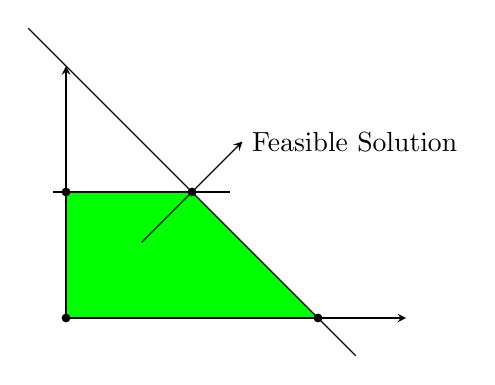
\begin{tikzpicture}[>=stealth,scale=1.6]
  \fill[green] (0,0) -- (0,1) -- (1,1) -- (2,0) -- cycle;
  \draw[->] (0,0) -- (0,2);
  \draw[->] (0,0) -- (2.7,0);
  \draw (-0.3,2.3) -- (2.3,-0.3);
  \draw (-0.1,1) -- (1.3,1);
  \draw[->] (0.6,0.6) -- (1.4,1.4);
  \node[right] at (1.4,1.4) {Feasible Solution};
  \fill (0,0) circle (1pt) (0,1) circle (1pt) (1,1) circle (1pt) (2,0) circle (1pt);
\end{tikzpicture}
\end{center}
\label{def:lp}
\dfn{Linear Program}{
A \emph{linear program (LP)} is the problem of finding values for $n$ variables
$x_1,x_2,\ldots,x_n\in\mathbb{R}$ that minimize (or equivalently, maximize) a given linear
objective function, subject to $m$ linear constraints
\begin{align*}
  \textbf{minimize:}\quad & \sum_{i=1}^n c_i x_i\\
  \textbf{Subject to:}\quad & \sum_i e_{i,j}x_i = b_j && \text{for } j=1,\ldots,m_1\\
  & \sum_i d_{i,k}x_i \ge g_k && \text{for } k=1,\ldots,m_2\\
  & \sum_i f_{i,p}x_i \le l_p && \text{for } p=1,\ldots,m_3
\end{align*}
where $m_1+m_2+m_3=m$.
}

\subsection*{Motivation}

Linear Programming is a very powerful tool -- it can be used in many applications, both
industrial and theoretical such as:
\begin{itemize}
  \item obtaining an optimal production plan to maximize a profit of a factory
  \item modeling network flow problems (what is maximum possible flow that doesn't exceed
    capacity of each connection)
  \item theory -- many theoretical problems can be introduced as Integer Programs (LP in which
    $x_i\in\mathbb{Z}$) that can be relaxed to LP obtaining a good approximation of optimal
    result -- we'll see such applications later in the course.
\end{itemize}

\subsection*{Solving Methods}

\paragraph{Simplex Method} was published by George Dantzig in 1947: it is the first complete
algorithm to solve linear programming problems.

The principle is the following: we start from an extreme point and then we look at its neighbors.
If one of these is better we move to it and continue in the same way, else we stop. Once we stop,
we can be sure that we have an optimal solution, since we're in a convex polytope. Even if it's
usually extremely fast, we know some bad examples where this method visits an exponential number
of extreme points before to reach a solution, so this method does not always run in polynomial
time.

\paragraph{Ellipsoid Method} was studied by Leonid Khachiyan in the seventies.

This method is guaranteed to run in poly time (exactly $\mathrm{poly}(n,m,\log(u))$ where $u$ is
the largest constant) but it is slow in practice.

We do a binary search for the optimal value of the objective function, so we can add the objective
function as a constraint, and just need to decide if there exists a feasible point. We start by
taking an ellipsoid surrounding the feasible area. We then check the center of the ellipsoid, if
it's inside the area then we have our solution, else we identify a violated constraint, and cut
our ellipsoid in two parts using this constraint, and construct a new ellipsoid around the part
of the old ellipsoid in which the constraint is satisfied. We repeat this process until we find a
feasible point or can be sure that the feasible area is empty.

\paragraph{Interior point Method} developed by Narendra Karmarkar in 1984. In this method we move
in the feasible region to find an OPT solution.

\subsection{Extreme Points}

Let us first define an extreme point:

\dfn{Extreme Point}{
A feasible solution is an \emph{extreme point} if it cannot be written as a convex combination of
other feasible solutions.
}

Just to recall:

\dfn{Convex Combination}{
A \emph{convex combination} of points $x_1,x_2,\ldots,x_n$ is a point of the form
$\sum_{i=1}^n\lambda_i x_i$ where the real numbers $\lambda_i$ satisfy $\sum_{i=1}^n\lambda_i=1$
and $\lambda_i\in[0,1]$ for all $i$.
}

Now, we state a theorem about extreme points. Extreme points are important because sometimes they
have useful structural properties, which we can exploit to design algorithms. We see two such
examples in this lecture.

\label{thm:extreme}
\thm{}{
If the feasible region is bounded, there always exists an optimum which is an extreme point.
}

\pf{}{
As the feasible region is bounded, there is an optimal solution $x^\star$ and any feasible point
can be written as a convex combination of the extreme points. In particular, we have
$x^\star=\sum_i\lambda_i x^{(i)}$ where $x^{(i)}$'s are feasible extreme points and $\lambda_i$'s
are non-negative real numbers satisfying $\sum_i\lambda_i=1$. Now let $c$ be the vector defining
the objective that we wish to maximize (the proof is the same if we minimize). Then we have
\[
  c^T x^\star = c^T\Big(\sum_i\lambda_i x^{(i)}\Big)=\sum_i\lambda_i c^T x^{(i)},
\]
which implies that there is an extreme point $x^{(i)}$ such that $c^T x^{(i)}\ge c^T x^\star$,
i.e., it is an optimal solution.
}

If the feasible region is not bounded, then we might not have any extreme points. For example, the
following LP does not contain any extreme points.
\begin{center}
\begin{tabular}{ll}
  Maximize   & $y$\\
  Subject to & $y\le 1$\\
             & $y\ge 0$
\end{tabular}
\end{center}

\begin{center}
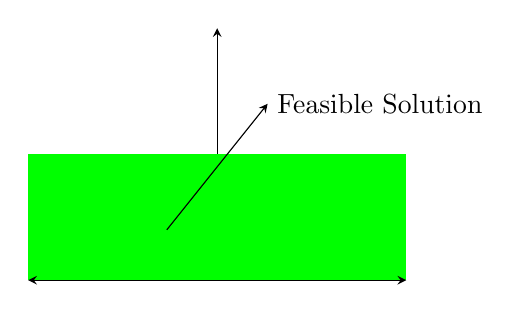
\begin{tikzpicture}[>=stealth,scale=1.6]
  \fill[green] (-1.5,0) rectangle (1.5,1);
  \draw[<->] (-1.5,0) -- (1.5,0);
  \draw[->] (0,1) -- (0,2);
  \draw[->] (-0.4,0.4) -- (0.4,1.4);
  \node[right] at (0.4,1.4) {Feasible Solution};
\end{tikzpicture}
\end{center}

\section{Examples}
\subsection{Maximum Weight Bipartite Perfect Matching}

In this section we are going to concentrate on maximum weight/profit bipartite perfect matching.
Given a bipartite graph $G=(V,E)$ with $V$ partitioned into $A$ and $B$ and edge-weights
$w:E\to\mathbb{R}$, this is the problem where we wish to find a perfect matching $M$ that
maximizes $w(M)=\sum_{e\in M}w(e)$. The LP for the
maximum weight bipartite perfect matching problem can be formulated as
\begin{center}
\begin{tabular}{ll}
  Maximize   & $\displaystyle\sum_{e\in E}x_e w_e$\\[8pt]
  Subject to & $\displaystyle\sum_{e=(a,b)\in E}x_e=1\quad\forall a\in A$\\[8pt]
             & $\displaystyle\sum_{e=(a,b)\in E}x_e=1\quad\forall b\in B$\\[8pt]
             & $x_e\ge 0\quad\forall e\in E$
\end{tabular}
\end{center}

In the linear program, we have a variable $x_e$ for each edge $e$ with the intended meaning that
it should take value $1$ if that edge is picked by the matching. The constraints say that each
vertex should have exactly one incident edge in the matching.

Note that in a feasible solution the variables $x_e$ may take values strictly between $0$ and $1$,
which does not really correspond to a matching. However, we have the following key structural
result:

\label{claim:integral}
\clm{}{}{
For bipartite graphs, any extreme point solution to the LP is integral.
}

\pf{}{
Let $x^*$ be an extreme point for the graph $G=(V_1,V_2,E)$ and let
$E_f=\{e\in E: 0<x^*_e<1\}$. Suppose towards contradiction that $E_f\neq\emptyset$. Note that
$E_f$ must then contain a cycle: indeed any vertex incident to an edge in $E_f$ is incident to at
least two edges in $E_f$. All these edges are fractional and we

\begin{center}
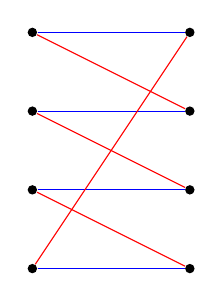
\begin{tikzpicture}[every node/.style={circle,fill,inner sep=1.2pt}]
  \foreach \i in {1,...,4} {
    \node (l\i) at (0,{4-\i}) {};
    \node (r\i) at (2,{4-\i}) {};
  }
  \foreach \i in {1,...,4} \draw[blue] (l\i) -- (r\i);
  \draw[red] (l1) -- (r2);
  \draw[red] (l2) -- (r3);
  \draw[red] (l3) -- (r4);
  \draw[red] (l4) -- (r1);
\end{tikzpicture}
\end{center}

want to define $y$ and $z$ so that they are feasible solutions and $x^*=\frac12(y+z)$ which will
contradict the fact that $x^*$ is an extreme point. Let $e_1,e_2,\ldots,e_{2k}$ be the edges of
the cycle. Let $y,z$ be
\[
  y_e=\begin{cases}
    x^*_e+\varepsilon & \text{if } e\in\{e_1,e_3,e_5,\ldots,e_{2k-1}\}\\
    x^*_e-\varepsilon & \text{if } e\in\{e_2,e_4,e_6,\ldots,e_{2k}\}\\
    x^*_e & \text{otherwise}
  \end{cases}
  \qquad
  z_e=\begin{cases}
    x^*_e-\varepsilon & \text{if } e\in\{e_1,e_3,e_5,\ldots,e_{2k-1}\}\\
    x^*_e+\varepsilon & \text{if } e\in\{e_2,e_4,e_6,\ldots,e_{2k}\}\\
    x^*_e & \text{otherwise}
  \end{cases}
\]
Notice that the degree constraints are still satisfied by $y$ and $z$ as we are alternating
between increasing and decreasing the edge values in a cycle of even length. Hence, to ensure
feasibility, we need to choose such a small $\varepsilon$ so as to guarantee that all $y_e$ and
$z_e$ are in $[0,1]$. For example $\varepsilon=\min\{x^*_e,(1-x^*_e): e\in E_f\}$ gives that both
$y$ and $z$ are feasible. Now one can easily see that $x^*=\frac12(y+z)$ which contradicts the
assumption that $x^*$ is an extreme point.
}

Because of the above claim, the polytope
\[
  P=\Big\{x: \sum_{b:(a,b)\in E}x_{(a,b)}=1\ \ a\in A,\ \ 
  \sum_{a:(a,b)\in E}x_{(a,b)}=1\ \ b\in B,\ \ x_{(a,b)}\ge 0\ \ (a,b)\in E\Big\}
\]
is called the \emph{bipartite perfect matching polytope}. Also, it says that we can solve the
maximum weight bipartite matching problem by simply solving the above linear program.

Unfortunately, the degree-constraints are not sufficient for general graphs which can be seen by
the following example:

\begin{center}
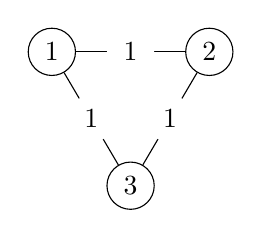
\begin{tikzpicture}[every node/.style={circle,draw,minimum size=6mm,inner sep=0pt}]
  \node (a) at (0,1.7) {1};
  \node (b) at (2,1.7) {2};
  \node (c) at (1,0) {3};
  \draw (a) -- node[draw=none,fill=white,midway,inner sep=1pt] {1} (b);
  \draw (a) -- node[draw=none,fill=white,midway,inner sep=1pt] {1} (c);
  \draw (b) -- node[draw=none,fill=white,midway,inner sep=1pt] {1} (c);
\end{tikzpicture}
\end{center}

Here, the solution that sets $x_e=1/2$ for every edge $e$ gives the optimal value $3/2$, but any
integral matching has only value $1$ (and the graph does not even have a perfect matching).

\subsection{Bipartite Vertex Cover}

Here, we consider minimum weight vertex cover on bipartite graphs. The definition of the vertex
cover problem is:

\dfn{Min Weight Vertex Cover}{
Given a graph $G=(V,E)$ with node-weights $w:V\to\mathbb{R}$ find a vertex cover $C$ (i.e.,
$e\cap C\neq\emptyset$ for all $e\in E$) that minimizes $w(C)=\sum_{v\in C}w(v)$.
}

\ex{}{
The minimum weight vertex cover (depicted in black) of the following graph is $3$ (obtained by
taking the vertices of weight $1$ and $2$).

\begin{center}
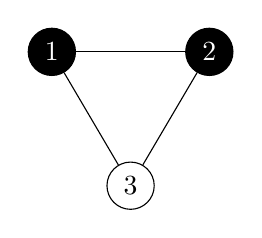
\begin{tikzpicture}[every node/.style={circle,draw,minimum size=6mm,inner sep=0pt}]
  \node[fill=black,text=white] (a) at (0,1.7) {1};
  \node[fill=black,text=white] (b) at (2,1.7) {2};
  \node (c) at (1,0) {3};
  \draw (a) -- (b);
  \draw (a) -- (c);
  \draw (b) -- (c);
\end{tikzpicture}
\end{center}
}

Similarly to the case of maximum weight bipartite perfect matching, we formulate a linear program
for the vertex cover problem. Here, we have a variable $x_v$ for each vertex $v$ with the intended
meaning that it takes value $1$ if that vertex is in the vertex cover. The constraints say that
each edge needs to be covered. The LP can be formulated as follows:
\begin{center}
\begin{tabular}{ll}
  Minimize   & $\displaystyle\sum_{v\in V}x_v w(v)$\\[8pt]
  Subject to & $x_u+x_v\ge 1\quad\forall\{u,v\}\in E$\\[4pt]
             & $0\le x_v\le 1\quad\forall v\in V$
\end{tabular}
\end{center}

We have the following structural result for bipartite graphs:

\label{claim:vc}
\clm{}{}{
For bipartite graphs, any extreme point to the vertex cover LP is integral.
}

\pf{}{
Consider an extreme point $x^*$ and let $V_f=\{v: 0<x^*_v<1\}$ be those vertices with fractional
values in $x^*$. Suppose toward contradiction that $V_f\neq\emptyset$. Further, let $A,B$ be the
bipartition of $V$ and let $A_f=V_f\cap A$ and $B_f=V_f\cap B$ be the fractional vertices in $A$
and $B$, respectively. As for bipartite matchings, we reach a contradiction by defining feasible
solutions $y$ and $z$ so that $x^*=\frac12(y+z)$ which contradicts that $x^*$ is an extreme point.
Let $\varepsilon=\min\{x_v,(1-x_v): v\in A_f\cup B_f\}$ and define $y$ and $z$ by
\[
  y_v=\begin{cases}
    x^*_v+\varepsilon & \text{if } v\in A_f\\
    x^*_v-\varepsilon & \text{if } v\in B_f\\
    x^*_v & \text{otherwise}
  \end{cases}
  \qquad
  z_v=\begin{cases}
    x^*_v-\varepsilon & \text{if } v\in A_f\\
    x^*_v+\varepsilon & \text{if } v\in B_f\\
    x^*_v & \text{otherwise}
  \end{cases}
\]
Clearly, we have that $x^*=\frac12(y+z)$. It remains to verify that $y$ and $z$ are feasible
solutions. Let us verify $y$ (the argument that $z$ is feasible is the same). By the selection of
$\varepsilon$, we have that $0\le y_v\le 1$ for all $v\in V$. We now need to verify that the
constraint for every edge is satisfied. Consider an edge $\{a,b\}\in E$ in the bipartite graph. We
need to verify that $y_a+y_b\ge 1$. If $x_a=1$ (or $x_b=1$), then we have that $y_a=1$ (or
$y_b=1$) and so the constraint holds. Otherwise $0<x_a,x_b<1$ and so $a\in A_f$ and $b\in B_f$.
This in turn implies that $y$ is feasible since
\[
  y_a+y_b=(x_a+\varepsilon)+(x_b-\varepsilon)=x_a+x_b\ge 1,
\]
where the last inequality holds because $x^*$ is a feasible solution.
}

The above structural result says that we can solve minimum weighted vertex cover on bipartite
graphs by simply solving the above linear program to find an optimal extreme point. It does not
work for general graphs which can be seen by considering the triangle (as for matchings). In
contrast to matchings, the vertex cover problem on general graphs is an NP-hard problem and we do
not expect to have efficient algorithms for it.

% \end{document}
